\documentclass[letterpaper,10pt]{article}
\usepackage[margin=2.5cm]{geometry}
\usepackage[utf8x]{inputenc}
\usepackage[T1]{fontenc}
\usepackage[spanish]{babel}
\usepackage{tabularx}
\usepackage{graphicx}

\newcommand{\swname}{Miau}
\newcommand{\swsub}{Manejadador gráfico de usuarios Linux}

\title{\swname \\ \swsub}
\date{\today}
\author{Israel Lozano \and Wilber Hinojosa \and Wilson Kassia} 

\begin{document}

\maketitle

\section{Introducción}
El sistema operativo Linux tiene como control de acceso a los grupos y usuarios; el control de acceso es a los archivos del sistema, directorios,
y dispositivos. Provee además métodos de control de accesos relativamente simples.

Al restringir  y/o permitir el acceso a las diferentes características 
de la computadora, es imperante se pueda realizar la \emph{ADministración de usuarios}.
De manera que se pueda determinar el comportamiento sobre la característica
del sistema que es ofrecida para permitir un funcionamiento seguro del sistema.

El concepto que caracteriza y determina a los sistemas Unix es: \emph{``Todo en Unix es un archivo''}
(Everything in Unix is a File). Lo que permite un paradigma unificado para el acceso
a un amplio rango de recursos de entrada y salida(impresores, archivos, teclados, etc).
Los sistemas Unix tienen desarrollado una abstracción para cumplir con el paradigma.

De manera que, cada archivo en Unix tiene como poseedor a un usuario y un grupo, y brinda 
tres tipos de acceso a éstos: 1)Lectura, 2)Escritura y 3)Ejecución.

\swname --\swsub-- es una aplicación gráfica, programada en Lenguage C, para la administración de los usuarios y grupos
en Linux utilizando las herramientas GLib para diferentes funciones de segundo plano y Gtk para
la presentación al usuario.

\section{Marco Teórico}
\subsection{Linux, usuarios y su administración }
La arquitectura del sistema operativo Linux puede ser visto desde dos niveles de ejecución, el nivel de usuario/aplicación
y el nivel del Kernel.
Existe una biblioteca (glibc) que hace de interface entre el nivel de usuario y el de kernel, y un mecanismo de transición 
entre ambas.
El usuario tiene acceso al espacio del Kernel sólo a través de una llamada al sistema(system call).

Un forma de acceso a un sistema linux es a través de una cuenta de usuario. Una sóla persona puede tener más de una cuenta,
siempre y cuando que utilicen una nombre diferente para cada uno. Hay algunos nombres de usuario que son reservados y
no pueden ser asignadas a un usuario convencional, tal es el caso de ``root''.

Las cuentas de usuario permiten y/o restringen la capacidad de una cuenta de usuario de utilizar algún recurso del sistema;
sean estas archivos, dispositivos, archivos de sistema, control sobre procesos, etc.

Los usuarios pueden ser agrupados dentro de un ``grupo'', y también agregados a grupos existentes para utilizar los privilegios
de acceso que se les asigna a éstos.
Los usuarios en sistemas Unix se identifican mediante un número único de usuario(User Id, UID) y un identifidor de grupo.

El paradigma de ``Todo en Unix es un archivo'' permite una abstracción unificada para el acceso a diferentes recursos
de entrada y salida. Por tanto, cada archivo en un sistema Linux tiene como propietario a un usuario y a un grupo para
permitir su utilización. Además, hay tres tipos de permisos de acceso: lectura, escritura y ejecución.
Diferentes permisos de acceso pueden ser aplicados a los propietarios de los archivos, a los grupos y a los ``otros''.

\noindent Para poder ver los permisos asignados a un archivo determinado se puede ejecutar el comando \emph{ls}:
\begin{verbatim}
$ ls -l 
-rw-r--r-- 1 root root 1087 Apr  6  2015 skeleton
-rwxr-xr-x 1 root root 4077 Mar 22  2015 ssh
-rwxr-xr-x 1 root root  731 Mar 11  2015 sudo
-rwxr-xr-x 1 root root 6581 Aug 29 11:17 udev
-rwxr-xr-x 1 root root  461 Aug 29 11:17 udev-finish
-rwxrwxr-x 1 kass kass 2737 Apr  6  2015 umountfs
-rwxr-xr-x 1 wil  wil  2202 Apr  6  2015 umountnfs.sh
-rwxr-xr-x 1 root root 1129 Apr  6  2015 umountroot
-rwxr-xr-x 1 root root 3111 Apr  6  2015 urandom

\end{verbatim}

La primera columna muestra los permisos asignados al archivo, la tercera el usuario al que pertenece y la cuarta
columna el grupo al que pertenece. Por ejemplo, el archivo \emph{umountfs} tiene los siguientes permisos:
\begin{itemize}
  \item Usuario: Lectura, escritura y ejecución (rwx). El usuario dueño del archivo puede realizar cualquier acción sobre este.
  \item Grupo: Lectura y ejecución (rx). Todos los usuarios pertenecientes al grupo ``kass'' pueden realizar cualquier acción sobre este archivo.
  \item Otros: Lectura y ejecución (rx). Cualquier otro usuario del sistema puede tener acceso al archivo pero no realizar ninguna modificación a este.
\end{itemize}
El archivo ``umountfs'' pertene al usuario ``kass'' y al grupo principal de éste.

\subsection{Tipos de usuario}
En Linux existen básicamente tres tipos de usuario a ser:
\subsubsection{El superusuario}
El usuario ``root'' o superusuario, o también llamado administrador del equipo, su UID es 0. Y es la única 
cuenta que cuenta con todos los permisos sobre los archivos del sistema, controla la administración de los usuarios y grupos.
Puede eliminar procesos independientemente del usuario, ejecutar tareas de mantenimiento del sistema,
instalar software, detener el sistema, modificar el kernel, etc.
Casi todos los archivos del sistema pertenecen a este usuario.

\subsubsection{Usuarios especiales}
Los usuarios: bin, daemon, adm, lp, sync, mail, operator, apache, etc. son usuarios especiales o cuentas del sistema.
No tienen ninguna equivalencia al usuario root pero tienen algunos privilegios especiales, tampoco presentan
contraseñas porque no necesitan iniciar sesión. En general, son creadas al momento de instalar el sistema operativo
o de algún programa de aplicación y se les asigna un número entre 100 y 999 (o lo definido en \emph{/etc/login.defs}.

\subsubsection{Usuarios normales}
Son las cuentas utilizadas para el uso común de un sistema con un directorio de trabajo asignado
para cada uno, que se ubica en el directorio ``/home''. Presentan privilegios completos dentro su directorio 
asignado. Se le asigna también un shell de inicio, un identificador de usuario, y un grupo principal, e incluir también grupos
adicionales a los cuales pueda acceder.

Los UID que se les asigna están en los rangos definidos generalmente en el archivo ``/etc/login.defs''; siendo entre 1000 y 60000
en Debian.

\subsection{Administración de los usuarios}
\label{sse:usersadmin}
Los sistemas Linux presentan herramientas que permiten realizar la administración de los usuarios y grupos.
Básicamente, trabajan sobre los archivos implicados en la administración de usuarios.
\subsubsection{Archivos implicados}
La siguiente tabla muestra los archivos implicados en la administración de los usuarios en Linux:\\
\begin{tabularx}{\textwidth}{ll}
Archivo & Propósito \\
\hline
/etc/shadow & Información de cuenta con el cifrado de contraseñas \\
/etc/passwd & Información de las cuentas de usuario \\
/etc/gshadow & Inforación de grupos con el cifrado de sus contraseñas \\
/etc/group & Información de los grupos del sistema al cual los usuarios pertenecen \\
/home/* & Directorio para alojar los espacios de trabajo de los usuarios \\

\end{tabularx}

\subsubsection{Adición de usuarios}
Para la adición de usuarios, hay un comando nativo llamado ``useradd'' que puede recibir únicamente el nombre del nuevo 
usuario a crear. Un nuevo usuario se puede crear con la siguiente llamada:
\begin{verbatim}
$ useradd -m -d /home/tso -s /bin/sh tso 
\end{verbatim}
Básicamente, va a crear un nuevo nuevo llamado ``tso'' con un entorno de trabajo en ``/home/tso'' y hará ejecutará
el shell ``/bin/sh''. Además, creará el directorio donde se ubicará el entorno de trabajo(parámetro -m).

Se pueden asignar explícitamente Id de usuario pero por recomendaciones del Sistema Operativo, es mejor dejar
que él mismo lo administre.


\subsubsection{Modificación de usuarios}
Para la modificación y/o actualización de información de usuarios ya existentes, el sistema Linux provee el comando \emph{usermod}.
Es posible modificar las mismas opciones que brinda el comando \emph{useradd}, como el nombre del usuario(login),
directorio ``home'', el shell, información en formato gecos, e inclusive el identificador de usuario.

\begin{verbatim}
$ usermod -s /bin/bash -d /home/tso2 -m -l tso2 tso
\end{verbatim}
Realiza un cambio de shell a ``bash''; luego, mueve el directorio de trabajo a \emph{/home/tso2} moviendo el contenido que había 
en el anterior entorno de trabajo(/home/tso) y cambia el nombre de inicio ``tso'' por ``tso2''.

Realizar una modificación al identificador del usuario no implica un cambio de los archivos creados por el usuario 
y que tengan el identificador previo. Es necesario hacer una búsqueda y actualización de los archivos anteriores.

Mediante este comando además es posibe modificar los grupos a los cuales va a pertenecer el usuario; se puede
incluir una lista nueva o añadir otro grupo más a los ya pertenecientes.
\begin{verbatim}
$ usermod -a -G grupito,grupito2,grupito3 tso2
\end{verbatim}
Lo que causa que el usuario tso2, aparte de los grupos a los cuales pertenece, también pertenezca a grupito, grupito2 y
grupito3(a causa del parámetro --append or -a).

\subsubsection{Eliminación de usuarios}
La eliminación de usuarios se realiza únicamente sobre los archivos de administración de usuarios.
El sistema Linux provee el comando ``userdel'' para realizar esta operación.

\begin{verbatim}
$ userdel -f -r tso2
\end{verbatim}

Realiza una eliminación del usuario tso2 dentro los archivos implicados en la administración de los usuarios.
La opción --remove(-r) elimina además del usuario, el directorio de trabajo de éste(/home/tso2); para eliminar archivos 
que no pertenezcan a éste usuario y/o es utilizado por otro usuario se debe incluir la opción --force(-f).

\subsubsection{Asignación de contraseña}
El comando de adición de usuarios(usermod), por defecto, no asigna contraseña al usuario, a menos que se utilice
el parámetro --password. Pero, el parámetro --password debe estar codificado y en el formato adecuado.
En tal situación se puede utilizar el comando \emph{chpasswd} de la siguiente manera:
\begin{verbatim}
$ echo ``tso2:elpoderdelmundo'' | chpasswd
\end{verbatim}
Se manda información al comando chpasswd a través de una tubería. La primera palabra es el nombre de usuario,
seguido por el śimbolo de dos puntos(:), posteriormente la contraseña sin necesidad de codificar.
Por defecto, el comando chpasswd hará el cifrado de la contraseña con el formato adecuado, 
y almacenará esta en el archivo /etc/shadow para un siguiente acceso por parte del usuario.

\subsection{Administración de grupos}
La administración de grupos consta de crear, eliminar, modificar y asignar usuarios para permitir o restringir el uso
de archivos a diferentes usuarios.

Un grupo es identificadora a través de un número identificador análogo al identificador de usuario. En este sentido,
el archivo /etc/login.defs determina cuáles son los rangos para la creación de grupos según sus tipos(de sistema o
normales).

En la creación de nuevos usuarios se añade por defecto un grupo con el mismo nombre del usuario creado. Además de éste, 
es posible crear otros grupos con el comando ``groupadd''. Y de la misma manera, éste grupo puede tener diferentes
usuarios dentro de él.
\begin{verbatim}
$ groupadd el_grupo
\end{verbatim}
Crea un nuevo grupo llamado ``grupito'' por defecto sin ningún usuario con él.
Al igual que los  usuarios, es posible añadir un identificador de grupo, pero es preferible que el mismo comando
le asigne uno automáticamente.

Para modificar el identificador o el nombre del grupo se utiliza el comando ``groupmod''.
\begin{verbatim}
groupmod -n grupito2 grupito
\end{verbatim}
Le modifica el nombre del grupo ``grupito'' a ``grupito2'' y se preserva el identificador acutal.

Finalmente, para eliminar un grupo es el comando ``userdel''; el cual sólo elimina el grupo de la lista
de grupos, no así los archivos que tengan este nombre de grupo.

\section{Lenguaje de programación y bibliotecas estándar}
El programa realizado será utilizando el lenguaje de programación C, utilizando las bibliotecas comunes estándar,
como ser: glibc.
Además, para facilitar la programación se hará uso de una biblioteca estándar desarrollada para el entorno de escritorio
Gnome; los cuales son: GLib, GObject y Gio. Este último grupo de bibliotecas también están disponibles
para entornos Microsoft Windows.

\subsection{Lenguaje C}
El lenguaje de Programación C fue desarrollado en los años 70 y es orientado a la implementación de Sistemas 
Operativos debido a su disponibilidad típica de estructuras de alto nivel como también de bajo nivel.
Es un lenguage muy popular para la programación de sistemas, como también para la creación de aplicaciones de usuario.

Los sistemas Unix están implementados en éste lenguage de programación.

No tiene un sistema de tipificación fuerte, lo que permite una flexibilidad bajo ciertos parámetros.
Pero, no tiene tipos de datos dinámicos que genera una reducción en la velocidad de desarrollo.

Un ejemplo de reducción de la velocidad de desarrollo es la de reservar y liberar memoria que debe realizarse
manualmente.

El proceso de compilación del lenguage C es el siguiente: 
\begin{enumerate}
  \item Preprocesado consistente en modificar el código fuente según las directrices determinadas para agilizar
    el proceso de compilación. Tal es el caso de reemplazar códigos definidos para diferentes constantes o
    directivas específicas para alguna plataforma.
  \item Compilación que genera el código objeto a partir del código ya procesado.
  \item Enlazado que unirá los códigos objeto de los módulos compilados y bibliotecas externas tanto estáticas
    como dinámicas que permita generar el programa final.

\end{enumerate}

\subsection{Bibliotecas estándar y multipropósito}
Para la implementación del programa, se han utilizado las siguientes herramientas que cumplen la portabilidad
entre diferentes plataformas, y debido al uso general en muchos bibliotecas de otro propósito, se harán
uso de éstas.
\subsubsection{glibc} Es la biblioteca estándar para C de GNU y distribuida bajo licencia GNU LGPL.
Esta biblioteca define y proporciona llamadas al sistema y funciones básicas como imprimir en pantalla,
escribir archivos, etc. Es altamente portable y se encuentra disponible para un gran variedad de 
arquitecturas. Glibc utiliza el estándar de programación ANSI C del año 1989, lo que le permite la portabilidad
entre diferentes plataformas y sistemas operativos.

El compilador \emph{gcc} utiliza por defecto esta biblioteca como la básica para la compilación.

\subsubsection{Glib}
Es una biblioteca de propósito general inicialmente desarrollado para el entorno Gnome, y Gtk.
Implmenta muchas funciones, tipos y estructuras no gráficas que permiten un desarrollo de programación
más amigables sobre glibc.
Presenta una abstracción independiente de cualquier sistema operativo y, por tanto, permite adaptarse
a diferentes situaciones. Consta de las siguientes características:
\begin{itemize}
  \item Tipos de datos estándar que no provee glibc, tal es el caso de listas enlazadas, colas, árboles.
    %También redefine tipos para poder facilitar la programación; tal es el caso de la definición
    %de un tipo ``gboolean'' que no existe en C estándar. A pesar de no tener mucha significancia
    %una rederefinición de un tipo de datos, éste brinda un entorno de programación más amigable.
  \item Introduce funciones para un mejor manejo de cadenas de caracteres.
  \item Añade funciones para la manipulación de archivos, suporte de internacionalización,
    advertencias, funciones para depuración, carga de módulos.
\end{itemize}

\subsubsection{GObject}
Es una biblioteca que provee una abstracción de un sistema de objetos y una interoperabilidad entre
diferentes lenguajes de manera transparente.
GObject es la biblioteca fundamental para la construcción del conjunto de sistema de objetos que consta
Gtk y todo el entorno Gnome. 

Implementa todas las características que determina el paradigma de Programación Orientada a Objetos
en un lenguage de programación estructurada como es el lenguaje C.

\subsubsection{GIO}
Es una biblioteca que provee una interfáz de programación para sistemas de archivos virtuales, como 
el acceso a archivos remotos, locales mediante diferentes protocolos de comunicación.
También tiene un soporte de transmisión asíncrona de archivos y utiliza el sistema de mensajes
DBus para la comunicación entre procesos.

Gio también es utilizado en la plataforma Gnome para las funciones de acceso a ficheros 
a través de diferentes protocolos.

\subsection{Bibliotecas para interfáz gráfica}
Al ser un sistema Linux la plataforma de trabajo, se hará uso de las funciones que provee
el sistema gráfico X Window System (X11). Pero, no se utilizará ninguna función primitiva 
explícitamente; sino que se aprovechará una biblioteca específica para la creación de interfaces 
de usuario que brinda diferentes elementos para interactuar con el usuario, el Gtk.

\subsubsection{Gtk+}
Es un biblioteca que contiene funciones y objetos para crear interfaces gráficas con el usuario,
a través de botones, paneles, menúes, pestañas, etc.

Gtk utiliza un sistema de objetos con base en GObject y debido a la portabilidad y conectividad 
de GObject es fácilmente portado como bibliotecas para otros lenguajes de progrmaación.

Gtk+ es todo un grupo de bibliotecas que permiten un acceso amigable, sencillo y accesible 
a las funciones gráficas que se presentan al usuario final.

\subsection{Herramientas útiles}
\subsubsection{GIT}
Un sistema de control de versiones que permitió a los estudiantes programar mediante 
la plataforma online github. El trabajo fue desarrollado cooperativamente usando estas herramientas.

\subsubsection{Gnu make}

\section{Metodología}
Para el desarrollo del software, se ha seguido la siguiente metodología:
\subsection{Recopilación de información de bibliotecas disponibles}
Se ha hecho la revisión de las bibliotecas para desarrollo de usuarios y grupos existentes,
en el cual se llegó a considerar si el programa se realizaría en modo texto o en un modo gráfico.

Se ha escogido el modo gráfico, utilizando Gtk+, debido a gusto personal nuestro y conocimientos previos.

Las bibliotecas a ser utilizadas fueron descritas previamente en la sección Marco Teórico.

\subsection{Estructuración del programa}
El programa fue escrito de manera que se evite en lo posible de ocultar las variables innecesarias
en el ámbito globar. Es decir, las únicas variables globales que se definieron son: lista de usuarios,
lista de grupos y lista de shells.
El resto de variables son constantes o tipos de datos de estructura, como ser identificación de columnas en las GtkTreeView
de usuarios y grupos, definición de UsersItem/GruopsItem.

Se mantiene un estilo de diseño de Modelo, Vista y Controlador (MVC) para la representación de los datos
con las facilidades que brinda el entorno de desarrollo de Gtk+.

\subsubsection{Definición de tipos de datos y estructuras}
Los usuarios son representados mediante una lista de doble enlace definida en Glib, al cual se añade como 
dato una estructura \_UsersItem previa definición de la estructura como un tipo de dato UsersItem.

\begin{verbatim}

Glist *users = NULL;
typedef struct _UsersItem UsersItem; //Definición del tipo de dato
struct _UsersItem { // Definición de la estructura
  uid_t uid; //Identificador del usuario. Si es nuevo se establece a 0 
  gid_t gid; //Identificador del grupo principal para el usuario
  char *name; //Nombre de usuario  o login
  char *fullname; //Nombre completo del usuario, primer parámetro de formato gecos
  char *shell; //Shell
  char * home; //Directorio de trabajo 
  gboolean is_new; //Variable para poder diferenciar los nuevos usuarios creados 
  gid_t *groups; //Lista de los id de grupos auxiliares a los que pertenece
  int n_groups; //Cantidad de grupos de la lista de grupos auxiliares
};

\end{verbatim}
El procedimiento con los grupos es similar con el tipo de dato GroupsItem.

Se añade además, las constantes para identificación de las columnas a ser mostradas, como ser:
\begin{verbatim}

enum {
  /*Identificación par la columna de ID*/
  UID_COL,
  /*Identificación para la columna de nombre o login*/
  UNAME_COL,
  /*Identificación para el nombre completo\*/
  UFULLNAME_COL,
  /*Columna de shell*/
  USHELL_COL,
  /*Columna de entorno de trabajo $home*/
  UHOMEPATH_COL,
  /*Columna de nuevo usuario*/
  UISNEW_COL,
  UN_COLS
};

\end{verbatim}

De la misma manera que con usuarios fueron definidas las columnas para los grupos.



\subsection{Funciones de segundo plano}
Después de la definición de las variables y estructuras, se han definido las funciones 
para rellenar éstos.
Las funciones realizan un lectura de los archivos \emph{/etc/passwd} y \emph{/etc/groups},
para usuarios y grupos, respectivamente, y llenar con ésta información, las estructuras
de datos definidas.

Las funciones \_populate\_users() y \_populate\_groups() realizan lo anteriormente descrito.

\begin{verbatim}
void _populate_users() {
  UsersItem *u;
  struct passwd *usr = NULL;
  /*Abre el archivo por defecto para la lectura de los usuarios.*/
  setpwent();
  usr = getpwent();
  while (usr != NULL) {
    u = NULL;
    u = (UsersItem *)(malloc (sizeof(UsersItem)));
    if (u != NULL) {
      if (usr->pw_uid >= 1000 && usr->pw_uid < 60000) {
        u->uid = usr->pw_uid;
        u->gid = usr->pw_gid;
        u->name = strdup(usr->pw_name);
        /*u->fullname = strdup(usr->pw_gecos);*/
        _parse_gecos(u, usr->pw_gecos);
        u->home= strdup (usr->pw_dir);
        u->shell = strdup (usr->pw_shell);
        u->is_new = FALSE;

        users = g_list_append (users, u);
        u->n_groups = 1;
        u->groups = malloc (sizeof(gid_t));
        
        /*Obtiene la lista de grupos auxiliares al que pertenec el usuario actual a ser leido
         * La primera vez, getgrouplist devuelve en el puntero de entero de entrada
         * en este caso n->groups la cantidad de grupos que realmente tiene el usuario
         * Para lo cual, una vez obtenido la cantidad total de grupos, se realiza una
         * segunda llamada con la memoria reservada para la cantidad total.
         */
        if (getgrouplist (u->name, u->gid, u->groups, &u->n_groups)) {
          g_free(u->groups);
          u->groups = malloc (u->n_groups * sizeof(gid_t));
          getgrouplist (u->name, u->gid, u->groups, &u->n_groups);
          g_print ("Group: %i\n", u->groups[1]);
        }
      }
    }
    usr = getpwent();
  }
  endpwent();
}
\end{verbatim}
La función setpwent() realiza la apertura y preparación del archivo \emph{/etc/passwd} 
para empezar a obtener la información de los usuarios. Después, se hace uso de la 
función getpwend() para obtener el primer uusario de la lista, seguidamente otra vez 
la función getpwent() para obtener el siguiente, hasta terminar. Una vez que se concluya
la obtención de los usuarios del archivo, se llama a la función getpwent() para que 
cierre archivo y libere los recursos de memoria que haya solicitado.

Para obtener la lista de grupos auxiliares, se llama a la función getgrouplist() que
devuelve en un espacio de memoria previamente reservado la información de los grupos a los
cuales pertenece el usuario.
Es importante aclarar que se debe asignar como parámetro, en la llamada a la función, el 
tamaño de memoria reservada para obtener los identificadores de grupos.
Posterior a la llamada, éste retorna en la misma variable la cantidad de grupos al que 
pertenece el usuario; motivo por el cual se realiza una liberación de los recursos
previos y se solicita una memoria con el tamaño requerido en función a la cantidad
de grupos devuelto.

De la misma manera que con usuarios, se obtiene la información para los grupos. 
Las funciones análogas para este caso son: setgrent(),getgrent() y endgrent().

Hay unas funciones auxiliares que se escribieron para facilitar el uso de las estructuras,
como la siguiente que muestra la información de un UsersItem en la salida estándar:
\begin{verbatim}
static void user_item_to_string (UsersItem *u) {
  g_print ("Id: %i, Name: %s, Home: %s, Shell: %s\n", u->uid, u->name, u->home, u->shell);
}
\end{verbatim}
La función anterior es por motivos nétamente de depuración.

Otra funciones son:
\begin{verbatim}
UsersItem * _find_by_id (uid_t id);
gboolean check_group(UsersItem *u, gid_t gid);
\end{verbatim}

Una vez que tanto las listas de grupos como de usuarios han sido obtenidos, 
se procede con el modelamiento de la información para la presentación al usuario.

\subsection{Modelo de datos para presentación}
Una vez que se ha definido y cargado la información para los usuarios y los grupos,
se procede a modelar la vista al usuario.

Gtk+ presenta unos objetos para trabajar el modelado que se adecúe al 
componente de visualización, uno de ellos es GtkListStore:

\begin{verbatim}

GObject
 |---GtkListStore

\end{verbatim}

Como la información a ser presentada no requiere más que una representación lineal,
se hará uso de ese Modelo. Los cuales serán creados mediante los métodos:
GtkTreeModel *create\_groups\_model y GtkTreeModel *create\_users\_model, para los 
modelos GtkListStore para grupos y usuarios; a los cuales se hace la carga de la información de las GList* users y groups:
\begin{verbatim}
static GtkTreeModel *create_users_model () {
  GtkListStore *model;
  GtkTreeIter iter;

  model = gtk_list_store_new (UN_COLS,
      G_TYPE_UINT,
      G_TYPE_STRING,
      G_TYPE_STRING, 
      G_TYPE_STRING,
      G_TYPE_STRING,
      G_TYPE_BOOLEAN
      );

  /* Se solicita la carga de los usuarios */
  _populate_users();
  GList *o_users = users;
  while(users != NULL) {
    UsersItem *usr = users->data;

    /* Se inserta en el modelo de datos, la información con las columnas
     * definidas anteriormente
     */
    gtk_list_store_append(model, &iter);
    gtk_list_store_set(model, &iter, 
        UID_COL, usr->uid,
        UNAME_COL, usr->name,
        UFULLNAME_COL,usr->fullname,
        USHELL_COL, usr->shell,
        UHOMEPATH_COL, usr->home,
        UISNEW_COL, usr->is_new,
        -1);
    /*tree_item_to_string(users->data);*/
    users = g_list_next(users);
  }
  /* Se preserva el origen de la lista de usuarios */
  users = o_users;
  return GTK_TREE_MODEL (model);
}
\end{verbatim}

El código anterior es similar para el llenado de la información para los grupos.
Con la diferencia que son menos columnas las que son solicitadas.

La ventaja principal que brinda GtkListStore es que tiene funciones ya implementadas
para el ordenamiento y búsqueda de la información, útil para que el usuario pueda 
hacer búsquedas rápidas en las listas que se le presentarán.

\subsection{Presentación de la información al usuario}
Se ha construido la estructura básica visual del programa utilizando la 
herramienta \emph{glade} en su versión 3. 

El programa, en su ventana principal, fue dividido en dos paneles(GtkBox), en el cual 
se incluyeron dos ventanas con capacidad de desplazamiento y una columna de botones(GtkButton).

En las ventanas con capacidad de desplazamiento, se adjunto el visor de información
para objetos que implementan la interfáz GtkTreeModel, como lo hace el objeto 
definido anteriormente para las listas(GtkListStore). Se incluyeron GtkTreeView para los usuarios y
para los grupos.

El cargado del diseño realizado utilizado \emph{glade} fue realizada con la biblioteca
GtkBuilder incluida en la versión 3 de Gtk+. Versiones anteriores requieren la utilización
de la biblioteca \emph{libglade}. Básicamente, las siguientes funciones permiten el 
cargado de la información y convertirlo en objetos Gtk para su uso:

\begin{verbatim}
  GtkBuilder *builder;
  /*Carga el diseño realizado utilizando glade*/
  builder = gtk_builder_new_from_file("um.glade");
  /*Recupera la referencia del objeto que fue construido previamente*/
  window = GTK_WIDGET(gtk_builder_get_object(builder, "main_window"));
  /*Añade las funcionalidades a los eventos */
  g_signal_connect (window, "delete-event", G_CALLBACK (on_delete_event), NULL);
  g_signal_connect (window, "destroy", G_CALLBACK (gtk_main_quit), NULL);
  /*Recupera la referencia al objeto que controla los GtkTreeView para usuarios y grupos*/
  users_tv = GTK_WIDGET(gtk_builder_get_object(builder, "treeview_users"));
  groups_tv = GTK_WIDGET(gtk_builder_get_object(builder, "treeview_groups"));

\end{verbatim}

Una vez cargado, se asignaron las funciones de respuesta a los diferentes eventos
que pudieran suceder en la interfáz, como ser: cerrar la ventana,
presionar click en el botón de añadir usuario, eliminar usuario, etc.

Debido a que el diseño creado con Glade se encuentra vacío, se realizó la carga
de la información y inclusión en los GtkTreeView respectivos. Inicialmente, 
se añadieron los modelos que utilizarán(gtk\_tree\_view\_set\_model) y,
posteriormente, se añaden las columnas que serán visualizadas; Las funciones: add\_columns y add\_groups\_columns se encargan de esa tarea.

Se aclara que los modelos que fueron añadidos, han sido cargados con la información 
previamente.

\begin{verbatim}
  gtk_tree_view_set_model (GTK_TREE_VIEW(users_tv), umodel);
  gtk_tree_view_set_model (GTK_TREE_VIEW(groups_tv), gmodel);

  add_columns(GTK_TREE_VIEW(users_tv), umodel, smodel);
  add_groups_columns(GTK_TREE_VIEW(groups_tv), gmodel);

\end{verbatim}

El uso de GtkTreeView ha permitido un rápido, fácil y sencillo manejo de la modificación
de la información, tal es el caso de la capacidad de edición de las diferentes celdas
y el control sobre éstas.

\subsection{Ejecución de las acciones solicitadas}
Las acciones desarrolladas para permitir el funcionamiento del programa, fueron
realizadas utilizando la función: g\_spawn\_sync definida en la biblioteca Glib.
\begin{verbatim}
gboolean
g_spawn_sync (const gchar *working_directory,
              gchar **argv,
              gchar **envp,
              GSpawnFlags flags,
              GSpawnChildSetupFunc child_setup,
              gpointer user_data,
              gchar **standard_output,
              gchar **standard_error,
              gint *exit_status,
              GError **error);
\end{verbatim}
La función ejecuta un proceso hijo de forma síncrona, de manera que espera su retorno 
para continuar con la ejecución.

Los comandos a ser ejecutados para brindar la funcionalidad al programa fueron definidos
en la sección \ref{sse:usersadmin}(Ver página: \pageref{sse:usersadmin}).

Se utilizó un pequeño trucho para ir añadiendo los parámetros para las diferentes opciones.
El cual es adjuntar un símbolo ``|'' entre opciones, esto debido a los problemas que 
generaron la utilización de comillas entre los parámetros. Después, se realizó una
separación de éstos con la función **g\_strsplit , que devuelve un arreglo de cadenas
de caracteres. Y los mismos son pasados como parámetros a la función que ejecutará
el comando.

\subsection{Compilación y ejecución del programa}
El programa escrito en lenguage C fue compilado con el compilador por defecto en sistemas
GNU Linux, el \emph{gcc}, haciendo uso de la herramienta \emph{pkg-config} para 
obtener rápidamente la dirección de las bibliotecas de cabeceras y de enlace para
las bibliotecas a ser utilizadas (Gtk+ y gio).
\begin{verbatim}
gcc -o um um.c \pikg-config --cflags --libs gtk+-3.0 gio-2.0`
\end{verbatim}

\section{Resultados}
Se obtuvieron los siguientes resultados:

\begin{figure}[htb]
  \centering
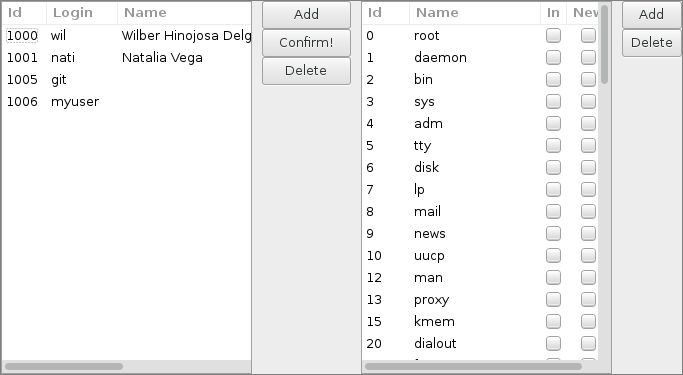
\includegraphics[scale=0.5]{pics/um000.png}
  \caption{Vista general de la interfáz del programa}
  \label{fig:main-window}
\end{figure}


\begin{figure}[htb]
  \centering
  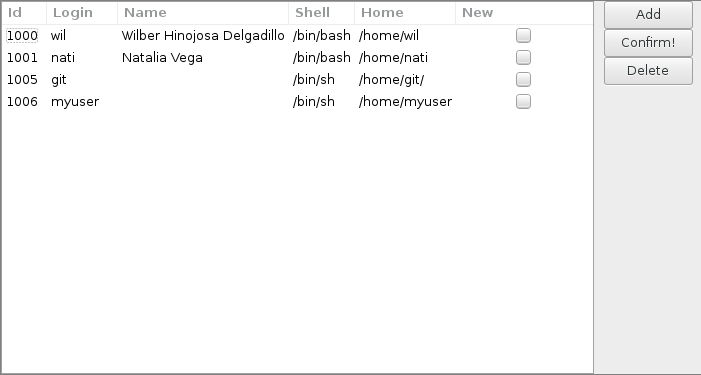
\includegraphics[scale=0.5]{pics/um001.png}
  \caption{Vista de todas las columnas del área de manejo de usuarios}
\end{figure}

\begin{figure}[htb]
  \centering
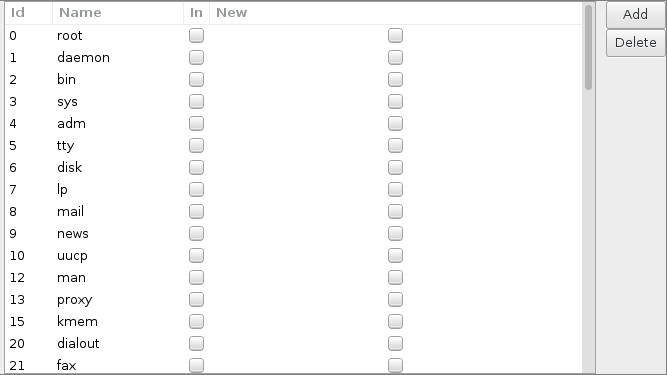
\includegraphics[scale=0.5]{pics/um002.png}
  \caption{Vista de todas las columnas del área de manejo de grupos}
\end{figure}


\section{Conclusión}
Se ha desarrollado una aplicación gráfica para la administración de usuarios y grupos
en sistemas Unix/Linux con las herramientas de desarollo de Glibc, Gtk+ y GLib principalmente y libgio 
como auxiliar. 

Se diseñó la interfáz utilizando herramienta de diseño de interfaces \emph{glade}.

El programa desarrollado permite crear, modificar, eliminar usuarios y grupos, y
asignar grupos de trabajo  a los diferentes usuarios.

Debido a los detalles que obligan a escribir y a la dependencia del sistema operativo,
se desestimó escribir el programa en sintaxis de C estándar.
\end{document}

